%%%%%%%%%%%%%%%%%%%%%%%%%%%%%%%%%%%%%%%%%
% University/School Laboratory Report
% LaTeX Template
% Version 4.0 (March 21, 2022)
%
% This template originates from:
% https://www.LaTeXTemplates.com
%
% Authors:
% Vel (vel@latextemplates.com)
% Linux and Unix Users Group at Virginia Tech Wiki
%
% License:
% CC BY-NC-SA 4.0 (https://creativecommons.org/licenses/by-nc-sa/4.0/)
%
%%%%%%%%%%%%%%%%%%%%%%%%%%%%%%%%%%%%%%%%%

%----------------------------------------------------------------------------------------
%	PACKAGES AND DOCUMENT CONFIGURATIONS
%----------------------------------------------------------------------------------------

\documentclass[
	letterpaper, % Paper size, specify a4paper (A4) or letterpaper (US letter)
	10pt, % Default font size, specify 10pt, 11pt or 12pt
]{CSUniSchoolLabReport}

\addbibresource{sample.bib} % Bibliography file (located in the same folder as the template)

%----------------------------------------------------------------------------------------
%	REPORT INFORMATION
%----------------------------------------------------------------------------------------

\title{Experiment Number 4\\State Variable Filter\\ EP3290} % Report title

\author{Chaganti Kamaraja Siddhartha\\EP20B012} % Author name(s), add additional authors like: '\& James \textsc{Smith}'

\date{\today} % Date of the report

%----------------------------------------------------------------------------------------

\begin{document}

\maketitle % Insert the title, author and date using the information specified above

\begin{center}
	\begin{tabular}{l r}
		Date Performed: & August 02, 2022 \\ % Date the experiment was performed
	\end{tabular}
\end{center}

% If you need to include an abstract, uncomment the lines below
%\begin{abstract}
%	Abstract text
%\end{abstract}

%----------------------------------------------------------------------------------------
%	OBJECTIVE
%----------------------------------------------------------------------------------------

\section{Objective}
Design a State Variable Filter which has a corner (natural undamped)
frequency, $f_C$ of 2.5 kHz and a quality factor, Q of 10. Assume both the frequency
determining resistors and capacitors are equal. Determine the filters DC gain and draw
the resulting circuit and Bode plot.
% If you have more than one objective, uncomment the below:
%\begin{description}
%	\item[First Objective] \hfill \\
%	Objective 1 text
%	\item[Second Objective] \hfill \\
%	Objective 2 text
%\end{description}

\subsection{Definitions}\label{definitions} % Labels provide a point for referencing, in this case with \ref{definitions} to refer to this subsection number

\begin{description}
	\item[State Variable Filter] The state variable filter is a type of multiple-feedback filter circuit that can produce all three filter responses, Low Pass, High Pass and Band Pass simultaneously from the same single active filter design. 
\end{description} 
\subsection{State Variable Filter Block Diagram}
\begin{figure}[H] % [H] forces the figure to be placed exactly where it appears in the text
	\centering % Horizontally center the figure
	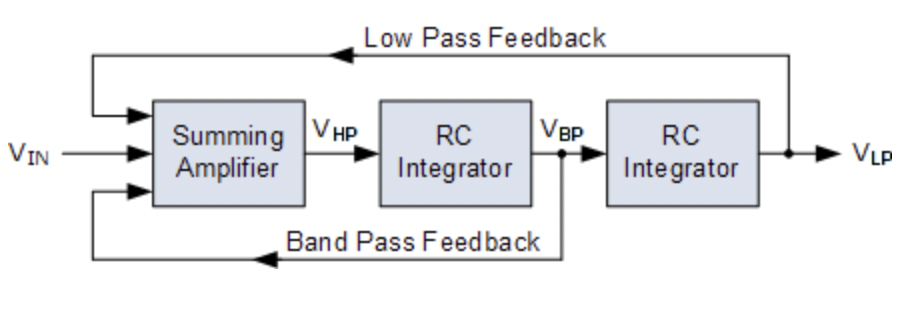
\includegraphics[width=0.65\textwidth]{blockdia} % Include the figure
	\caption{State Variable Filter Block Diagram}
\end{figure}
\subsection{State Variable Filter Circuit}
\begin{figure}[H] % [H] forces the figure to be placed exactly where it appears in the text
	\centering % Horizontally center the figure
	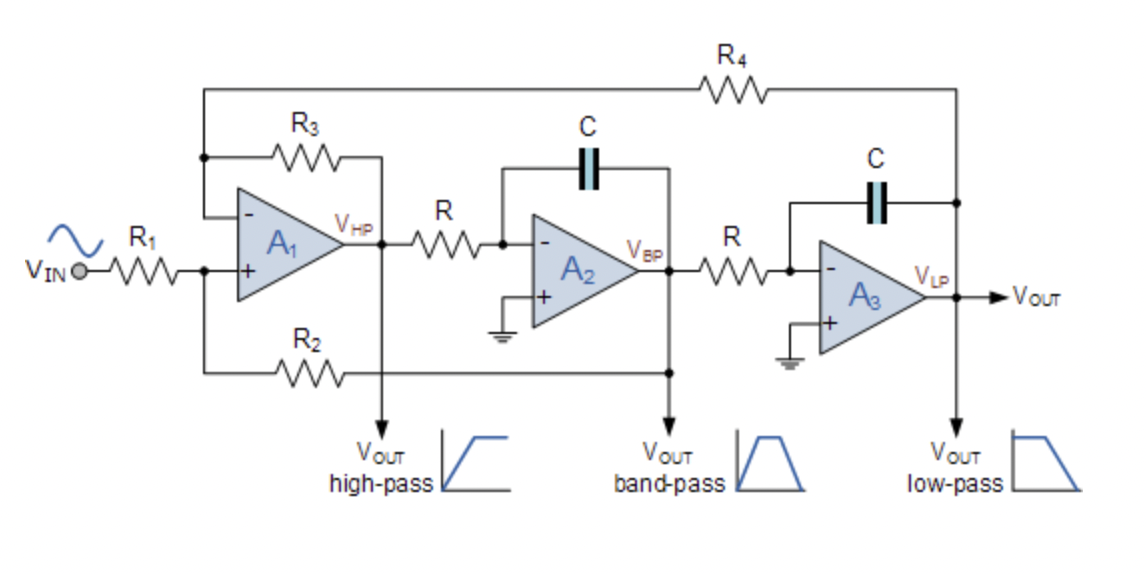
\includegraphics[width=0.65\textwidth]{svfc} % Include the figure
	\caption{State Variable Filter Circuit}
\end{figure}
\subsection{Normalized response of a State Variable Filter}
\begin{figure}[H] % [H] forces the figure to be placed exactly where it appears in the text
	\centering % Horizontally center the figure
	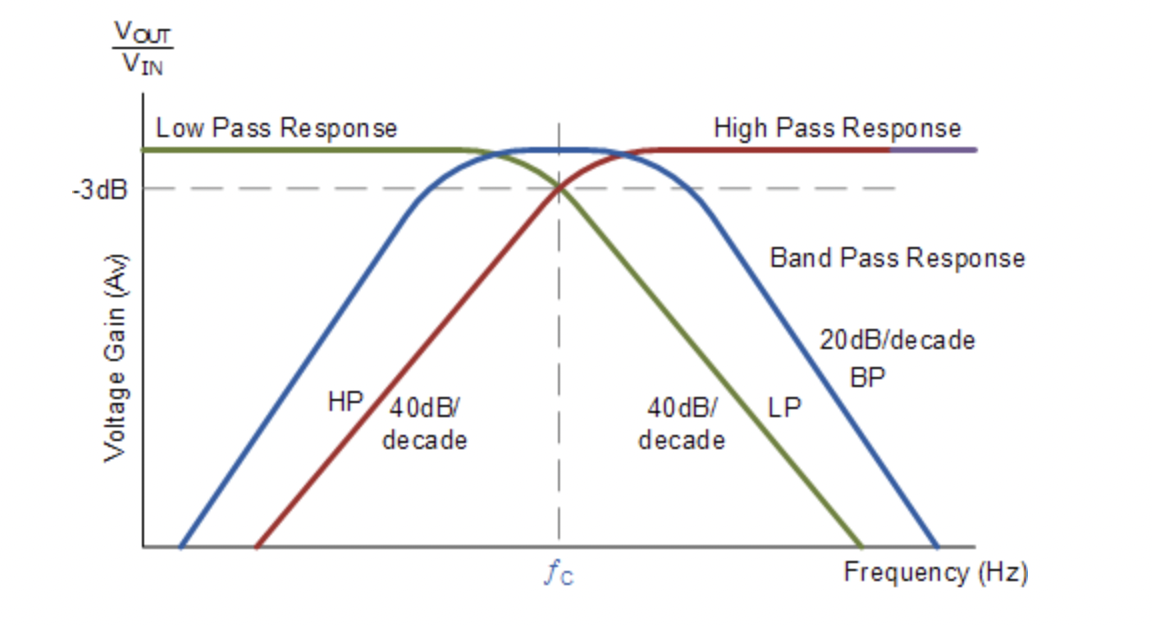
\includegraphics[width=0.65\textwidth]{nrsv} % Include the figure
	\caption{Normalized response of a State Variable Filter}
\end{figure}
\section{Calculations}
\subsection{Op-amp Integrator Circuit}
\begin{figure}[H] % [H] forces the figure to be placed exactly where it appears in the text
	\centering % Horizontally center the figure
	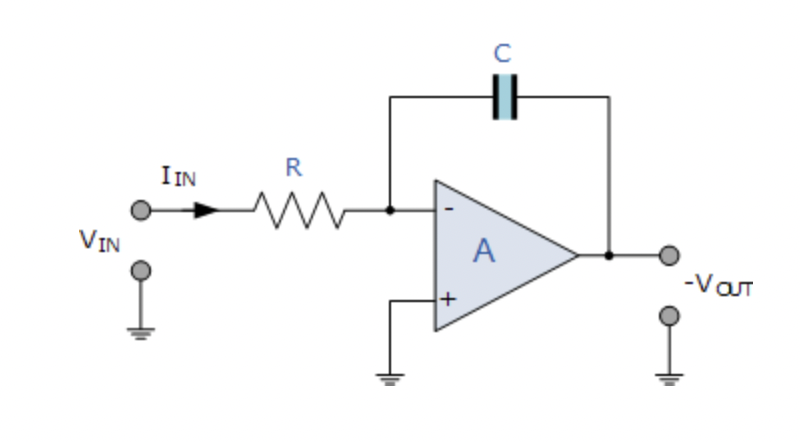
\includegraphics[width=0.65\textwidth]{inte} % Include the figure
	\caption{Op-amp Integrator Circuit}
\end{figure}
\begin{gather}
	V_{out} = -\frac{1}{RC}\int_{0}^{t} V_{IN}dt \\
	V_{out} = -\frac{1}{2 \pi f_c RC} V_{IN} 
\end{gather}
The output voltage $V_{out}$ is a constant 1/RC times the integral of the input voltage Vin with respect to time. Integrators produce a phase lag with the minus sign (-) indicating a $180^\circ{}$ phase shift because the input signal is connected directly to the inverting input terminal of the op-amp.
In the case of op-amp A2 above, its input signal is connected to the output of the proceeding op-amp, A1 so its input is given as $V_{HP}$ and its output as $V_{BP}$. Then from above, the expression for op-amp, A2 can be written as:
\begin{equation}
	V_{BP} = -\frac{1}{2 \pi f_c RC}V_{HP}  
\end{equation}
\subsection{Op-amp A2 Transfer Function} 
\begin{equation}
	\frac{V_{out} }{V_{IN} } = \frac{V_{BP} }{V_{HP} } = -\frac{1}{2 \pi f_c RC} 
\end{equation}
\subsection{Op-amp A3 Transfer Function} 
Exactly the same assumption can be made as above to find the transfer function for the other op-amp integrator, A3
\begin{equation}
	\frac{V_{out} }{V_{IN} } = \frac{V_{LP} }{V_{BP} } = -\frac{1}{2 \pi f_c RC} 
\end{equation}
So the two op-amp integrators, A2 and A3 are connected together in cascade, so the output from the first $(V_{BP})$ becomes the input of the second. So we can see that the band pass response is created by integrating the high pass response and the low pass response is created by integrating the band pass response. Therefore the transfer function between $V_{HP}$ and $V_{LP}$ is given as:
\begin{equation}
	\frac{V_{LP} }{V_{HP} } = -\frac{1}{2 \pi f_c RC} X -\frac{1}{2 \pi f_c RC} =\frac{1}{(2 \pi f_c RC)^2}   
\end{equation}
\subsection{Amplifier Summing Circuit}
 
Operational amplifier, A1 is connected as an adder-subtracter circuit. That is it sums the input signal, $V_{IN}$ with the $V_{BP}$ output of op-amp A2 and the subtracts from it the $V_{LP}$ output of op-amp A3, thus 
\begin{gather}
	i_1 = \frac{V_{IN}-(+V) }{R_1}+\frac{V-V_{BP} }{R_2} = 0\\
	\implies V = \frac{V_{IN}R_2 + V_{BP}R_1 }{R_1 + R_2}
\end{gather}
and 
\begin{gather}
	i_2 = \frac{V_{HP}-(-V) }{R_3}+\frac{-V-V_{LP} }{R_4} = 0\\
	\implies -V = \frac{V_{LP}R_{3}  + V_{HP}R_4 }{R_3 + R_4}
\end{gather}
From equations (5), (6), (8), (10)
\begin{equation}
	\boxed{\frac{V_{OUT}}{V_{IN}} = \frac{V_{LP} }{V_{IN} } = \frac{\frac{R_2(R_3 + R_4)}{R_3(R_1 + R_2)}X\frac{1}{RC}}{\frac{R_3}{R_4 R C}+\left(\frac{R_2(R_3 + R_4)}{R_3(R_1 + R_2)}X\frac{1}{RC}\right)+\left(\frac{1}{2 \pi f RC}\right)^2}}
\end{equation}
\subsection{Normalized 2nd-order Transfer Function}
\begin{equation}
	\boxed{\frac{V_{OUT} }{V_{IN} } = \frac{A_o\left(\frac{f}{f_o}\right)}{1+2\zeta \frac{f}{f_o}+ \left(\frac{f}{f_o}\right)^2}}
\end{equation}
\subsection{State Variable Filter Corner Frequency}
\begin{equation}
	f_{c(HP)} = f_{c(BP)} = f_{c{LP}} = \frac{1}{2\pi RC}
\end{equation}
\subsection{Q-Factor of a state variable Filter}
 \begin{equation}
	Q = \frac{1}{2 \zeta} = \frac{R_4(R_1 + R_2)}{R_1(R_3 + R_4)}\sqrt{\frac{R_3}{R_4}X \frac{RC}{RC}} 
 \end{equation}
Objective $f_c = 2.5 kHz$ and $Q = 10$, 
using equation (13) and fixing C = 10nF, to find R\dots
\begin{equation}
	R = \frac{1}{2 \pi f_c C} = \frac{1}{2 \pi X 2500 X 10 nF}= 6.33 k\Omega
\end{equation}
Taking $R_3 = R_4 = 10 k\Omega$ and using equation (14), to find $R_1 $ and $R_2$\dots
\begin{equation}
	10 = \frac{10(R_1 + R_2)}{R_1(10 + 10)} \implies  \frac{R_2}{R_1} = 19. 
\end{equation}
Taking \(R_1 = 1 k\Omega\) and \(R_2 = 19 k\Omega\) 
\section{State Variable Filter Design}

\begin{figure}[H] % [H] forces the figure to be placed exactly where it appears in the text
	\centering % Horizontally center the figure
	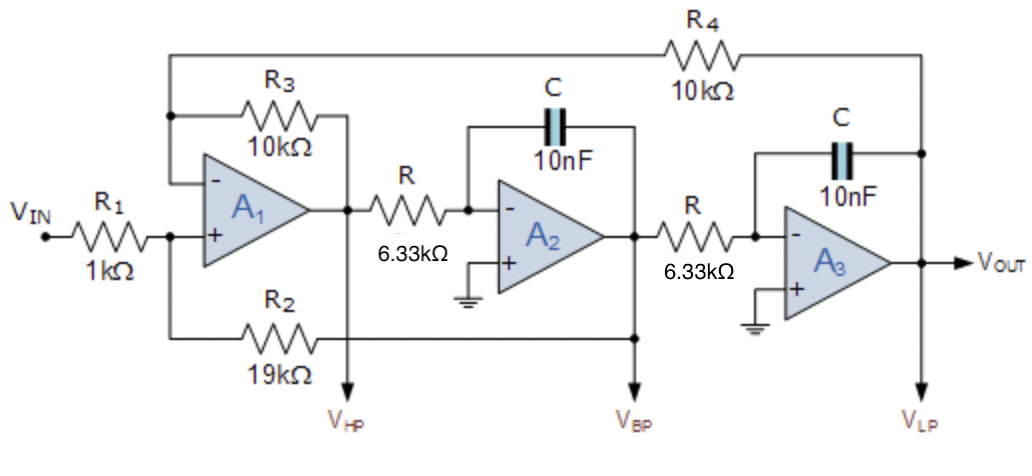
\includegraphics[width=0.65\textwidth]{svf} % Include the figure
	\caption{State Variable Filter Design}
\end{figure}
%----------------------------------------------------------------------------------------
%	EXPERIMENTAL DATA
%----------------------------------------------------------------------------------------

\section{Experimental Data}

\begin{figure}[H] % [H] forces the figure to be placed exactly where it appears in the text
	\centering % Horizontally center the figure
	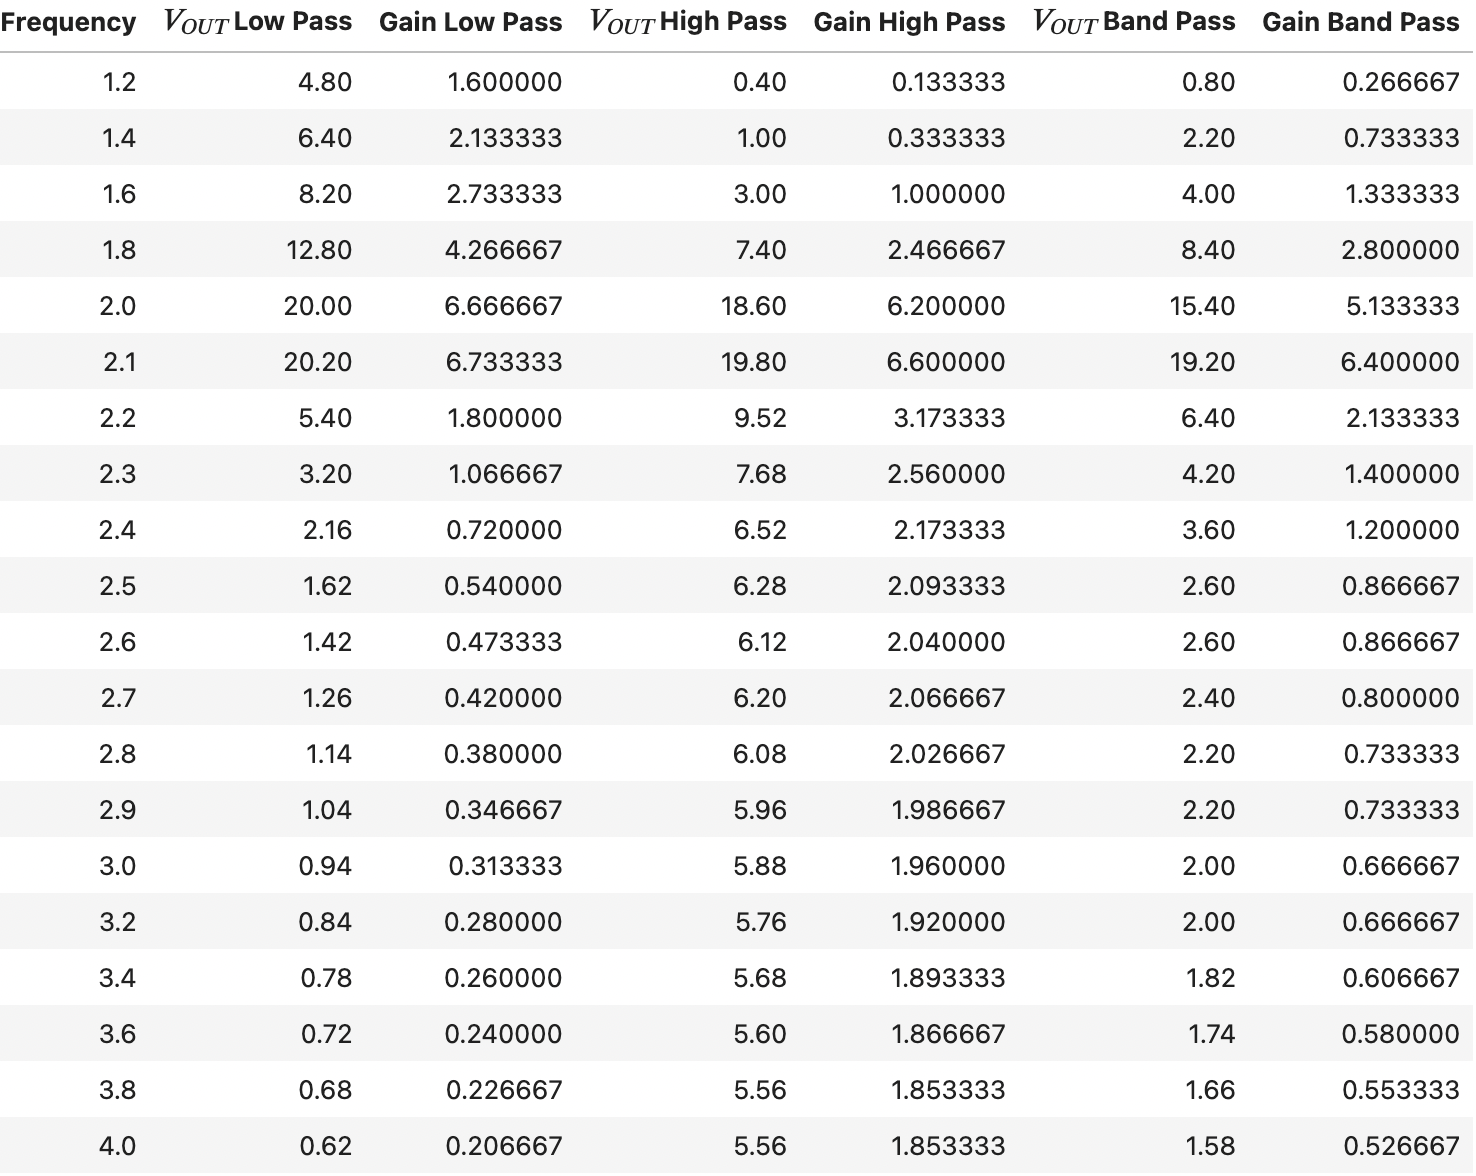
\includegraphics[width=0.65\textwidth]{data} % Include the figure
	\caption{Experimental Data}
\end{figure}
\section{Results and Conclusions}
\begin{figure}[H] % [H] forces the figure to be placed exactly where it appears in the text
	\centering % Horizontally center the figure
	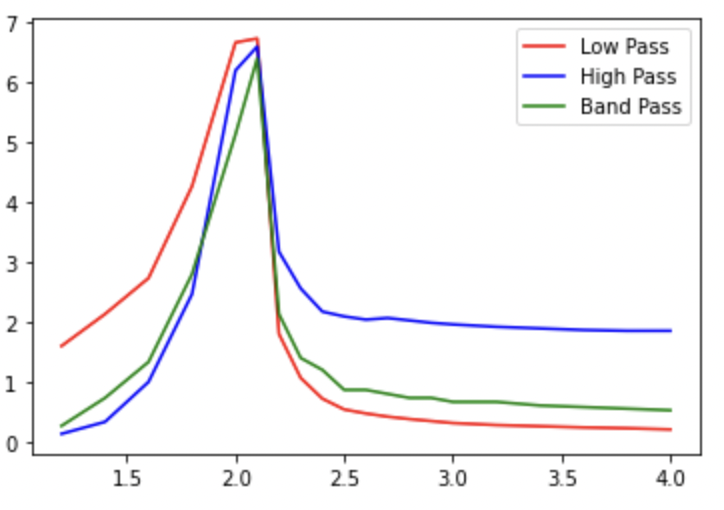
\includegraphics[width=0.65\textwidth]{graph} % Include the figure
	\caption{Bode Plot of Gain Vs Frequency}
\end{figure}
The cut-off frequency of Low-Pass, Band-Pass and High-Pass are approximately equal. The frequency is near to 2.5kHz but not exactly equal due to some fault in resistor values and capacitor values etc. 

%----------------------------------------------------------------------------------------
%	SAMPLE CALCULATION
%----------------------------------------------------------------------------------------

\end{document}